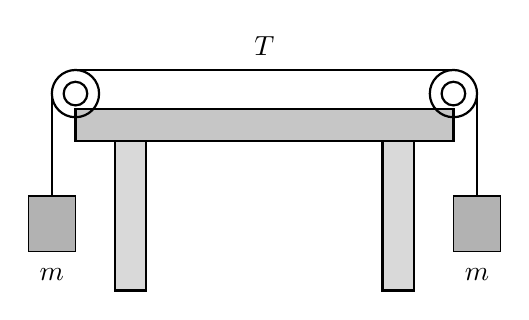
\begin{tikzpicture}
  % table top
  \draw[thick, fill=gray!45] (0.6,1.9) rectangle (5.4,2.3);
  % table legs
  \draw[thick, fill=gray!30] (1.1,0) rectangle (1.5,1.9);
  \draw[thick, fill=gray!30] (4.5,0) rectangle (4.9,1.9);
  % pulleys at each end
  \draw[thick] (0.6,2.5) circle (0.3);
  \draw[thick] (0.6,2.5) circle (0.15);
  \draw[thick] (5.4,2.5) circle (0.3);
  \draw[thick] (5.4,2.5) circle (0.15);
  % string over the top, T label
  \draw[thick] (0.6,2.8) -- (5.4,2.8);
  \node at (3.0,3.1) {$T$};
  % strings down to hanging masses
  \draw[thick] (0.3,2.5) -- (0.3,1.2);
  \draw[thick] (5.7,2.5) -- (5.7,1.2);
  \draw[fill=gray!60] (0.0,0.5) rectangle (0.6,1.2);
  \node at (0.3,0.2) {$m$};
  \draw[fill=gray!60] (5.4,0.5) rectangle (6.0,1.2);
  \node at (5.7,0.2) {$m$};
\end{tikzpicture}
